O funcionamento da máquina assíncrona pode ser representado utilizando um ímã permanente e um disco livre para girar, como mostrado na figura \ref{fig:13}.

\begin{figure}[ht!]
\center 
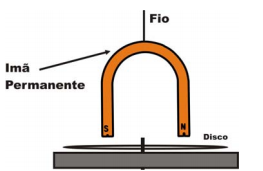
\includegraphics[scale=1.2]{imagens/13.PNG}
\caption{Princípio de funcionamento da máquina assíncrona.}\label{fig:13}
\end{figure}

O ímã permanente é suspenso sobre um disco metálico. O fluxo magnético produzido pelo ímã permanente flui através do circuito magnético composto pelo ímã permanente, os entreferros e a placa de ferro. Ao girar o ímã permanente, o disco que se encontra sob o ímã também gira. O disco acompanha o movimento de rotação do ímã permanente devido à circulação de correntes induzidas. Estas correntes são induzidas devido ao movimento relativo entre o disco e o ímã permanente. As correntes induzidas tendem a produzir, de acordo com a lei de Lenz, um polo sul magnético no disco sob o polo norte magnético girante do ímã permanente, assim como um polo norte magnético no disco sob o polo sul magnético girante do ímã permanente. Enquanto o ímã continua seu movimento em relação ao disco, continuará a indução de correntes parasitas e polos magnéticos com polaridades opostas. O disco, desta forma, gira no mesmo sentido que o ímã permanente, mas deve girar a uma velocidade menor para que haja uma velocidade relativa entre o ímã permanente e o disco metálico.

